\chapter{Related Work}
\label{cha:theory}

This section covers related work on arrival time prediction 
and motion pattern modeling using spatio-temporal data. It
also covers related work relevant to clustering of trajectory data
and event detection in motion patterns.

\section{Arrival Time Prediction}
Arrival time prediction is, in a nutshell, the problem of answering
the question ``When does the bus arrive?''. Formally, the goal is to
learn a function $t = f(x)$ for arrival time $t$ and some vector $x$, which
contains information on the current state of the world. For instance, it
could contain the position of the closest vehicle and the time of day.
In recent years, machine learning techniques have been very successful
at predicting the arrival time with small errors, and Long Short-Term 
Memory Networks (LSTMs) in particular have proven
extremely effective. J. Pang et al. predicted bus arrival times to the next station in a
continuous setting using LSTMs given the current position of a bus and static domain knowledge
about its last stop~\cite{pang2018learning}.
D. Nguyen et al. also used LSTMs, but with entire
trajectories~\cite{Nguyen2018Jun}. They predicted arrival times of
ships by training a model to generate continuations of trajectories, and  
when the model was presented with a new unfinished trajectory, it generated a
probable continuation until it arrived at a port. This was then used to
prediction both the destination and the arrival time.

While these approaches do perform admirably with respect to accuracy, 
they lack explainability and a way to quantify prediction uncertainty.

\section{Motion Pattern Learning}
Motion pattern learning is the problem of learning motion patterns from a
set of trajectories, such that each pattern captures a different
characteristic of the trajectories. An example with synthetic data can be
seen in Figure~\ref{fig:motion-pattern-example}. Note that the term
\textit{trajectory learning} is often used in the literature for the
same problem, however, the term ``trajectory'' is ambiguous so in the
context of this thesis the name motion pattern learning will be used. 
\begin{figure}[H]
  \centering
  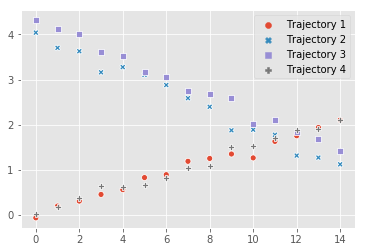
\includegraphics[width=0.7\textwidth]{figures/motion-pattern-example}
  \caption{Synthetic data showing two motion patterns with two trajectories in
    each. Trajectory 2 and 3 belong to one motion pattern and
    Trajectory 1 and 4 belong to a second motion pattern.}\label{fig:motion-pattern-example}
\end{figure}
Motion pattern learning has a natural interpretation as a
clustering problem, but clustering trajectories is difficult,
since different trajectories can have different lengths.
This means that they do not exist in the same vector space and are not
naturally comparable using similarity metrics based on Euclidan
distance. Because of this, more advanced similarity metrics often need to be used. 

\subsection{Trajectory Similarity Metrics}\label{sec:traj-sim-metrics}
There are several ways to construct a similarity metric for
trajectories. Some widely-used metrics are Euclidan distance,
Dynamic Time Warping (DTW), Longest Common Sub-Sequence (LCSS), and Edit
Distance (ED)~\cite{Wang2013Jan}. DTW and LCSS have seen use in
motion pattern learning~\cite{Tang2018Aug, Vlachos2002Feb}, but suffer
from high time-complexity, making them unsuitable for real time processing~\cite{Zhang2006Aug}
An alternative to previously mentioned similarity metrics are probabilistic
approaches, where models are fit to trajectories
and similarity is measured as data likelihood~\cite{Kim2011Nov, Tran2014Jun, Tiger2015Jul}.
One advantage of a probabilistic approach are that it is not limited by
purely spatial information, since any information about the trajectories can
be modeled. For instance, spatial position could be combined
with velocity and acceleration.

\subsection{Probabilistic Approaches}
The probabilistic approach to trajectory learning assumes a model for each motion pattern
and infers its parameters from data. This is incredibly similar to how
probabilistic models are used to create similarity metrics, but instead this
is done for a cluster of trajectories. Two popular approaches for this
is GPs and hierarchical Bayesian models.

\subsubsection{Gaussian Processes}
GPs have been used in several domains for modeling trajectories.
M. Pimentel et al. used GPs to model the vital signs of patients~\cite{Pimentel2013Sep}, 
and were successfully able to cluster the data using hierarchical clustering
and the GP model likelihoods. They then modeled the motion pattern
for a cluster as a GP with the average mean and variance for all GPs in it.
K. Kim. et al. used GPs to model the motion patterns of cars from
surveillance camera~\cite{Kim2011Nov}. They introduce the
concept of a \textit{frame}, in which the trajectories are
discretisised before fitting GPs to them. Having discrete trajectories meant that
the local likelihood for observed data $x_t, y_t$ in time step $t$
could be computed as $P(y_t | x_t, {M_k})$ for model $M_k$, which
were aggregated to compute a global similarity metric $L_k$,
which in turn was used to cluster the trajectories. To compute the motion
patterns of clusters, a sampling scheme was used. In each time
point, three GPs were drawn uniformly without replacement from the
cluster. The mean value of all drawn GPs were then used as data points
to fit a GP for the clusters motion pattern.

Q. Tran and J. Firl used data with both spatial position and velocity,
and used GPs to model a vector field for each observed
trajectory~\cite{Tran2014Jun}. Before GPs were trained, the trajectories 
were normalised using spline interpolation and a
sampling scheme. They did not perform any clustering. Instead, they
constructed their motion patterns by driving their own test vehicle. 
When presented with a new trajectory, the model could compute the most
likely motion pattern, and use a particle filter for the vector
field to predict continuations of motion patterns. 

The work of M. Tiger and F. Heintz aimed to improve upon the approach of K. Kim et
al. who had implicitly assumed that all trajectories were generated
from one underlying processes~\cite{Tiger2015Jul}. Doing so causes the model to
underestimate its variance, which in turn causes the models likelihood
to be too small for data that should be considered likely. To avoid this,
sets of trajectories were modeled as a
mixture-of-Gaussian-processes (MoGP). They then considered ``slices''
of trajectories, orthogonal to progression, which were approximated as
Gaussian distributions. The posterior of these approximations was
then assumed to come from a single GP, which was approximated on synthetic data, 
a process they call \textit{inverse Gaussian process regression}.
M. Tiger and F. Heintz also suggested an improvement on
the vector field approach proposed by Q. Tran and
J. Firl~\cite{Tiger2018Jun}, in which they use GPs for the functions
$(x, y) \mapsto \tau \mapsto x, y, x', y'$ for $\tau = [0, 1]$, compared to
$(x, y) \mapsto x', y'$ used by Q. Tran and J. Firl. Their approach
was shown to perform better in benchmarks.

C. Leysen et al. also aim to improve on the work of K. Kim et
al~\cite{Leysen2016Sep}. Instead of fitting a GP to re-sampled trajectories, 
they simply select the trajectory in a cluster which maximises the overall
likelihood of the data points in the cluster. Their approach still
assumed a single underlying function for all trajectory data,
and consequently still underestimated model variance.

\subsubsection{Hierarchical Bayesian Models}
The idea behind hierarchical Bayesian models used for trajectory
learning is borrowed from the natural language processing field, where
they are known as topic modeling. Topic modeling are unsupervised
techniques for clustering documents into different topics, and by 
considering spatio-temporal trajectories as documents,
their observations as words, and the motion patterns they belong to as
topics, the same techniques can be used to model motion pattern.  
These models are usually based on Latent Dirichlet Allocation (LDA) or
a generalisation thereof known as Hierarchical Dirichlet Process (HDP)
introduced by Teh et al.~\cite{teh2005sharing}, which are both so called \textit{bag-
of-words}-models. A bag-of-words-model assumes independence between
words in a document, which in the domain of trajectories translates to the
assumption that observed data points are independently drawn.

Both LDA and HDP require a set amount of clusters, which is a great
weakness. Wang et al. proposed a model called \textit{Dual Hierarchical Dirichlet
Process} (Dual-HDP)~\cite{Wang2008Jun}, which improves upon the HDP model
by allowing the model to learn the number of topics and documents from
data. Zhou et al. further improved upon HDP and LDA by using Markov random
fields to encode prior beliefs in a model called \textit{Random Field
  Topic} (RFT)~\cite{Zhou2011Jun}.

\section{Event Detection}
In the context of motion patterns and trajectory data, event detection
can be seen as the problem of finding patterns in time
series. For this, convolution can be used with specific convolution
kernels corresponding to the event of interest~\cite{smith1997scientist}.

Duvenaud et al. explored a different approach, where they modeled
time series as GPs with a composite kernel~\cite{duvenaud2013structure}. To construct the
kernel they greedily searched over different kernel structures,
and composed kernel functions to maximise the marginal likelihood.
The structure of the resulting kernel could then be analysed to reveal
characteristics of the time series.